\chapter{{\LaTeX}\ Specific Usage}

This template is heavily built on \href{https://www.ctan.org/pkg/memoir}{memoir} package. See memoir's documentation for detailed usage.

\section{Figures}
Common file formats (PDF, PNG, and JPG) are supported. Vector figures should use PDF to ensure the resolution, such as \fref{fig:vector}.

\begin{figure}[tbh]
  \centering
  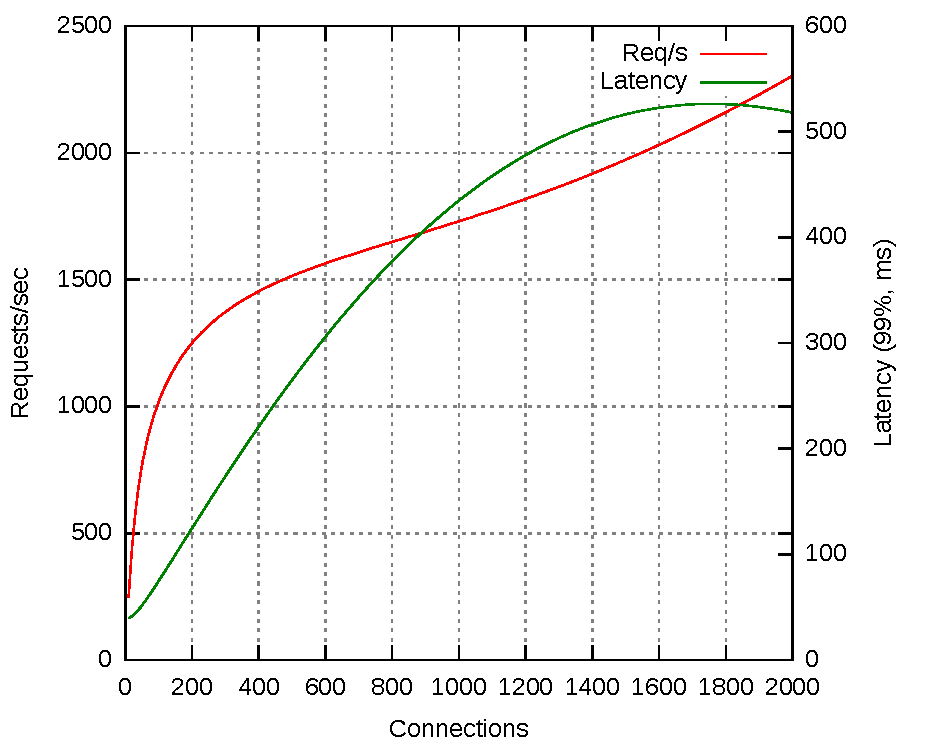
\includegraphics[width=0.6\textwidth]{figures/just-a-plot}
  \caption{Example vector figure in PDF.}
  \label{fig:vector}
\end{figure}

\section{Subfigures and subtables}
Powered by \texttt{subcaption} package.
See Figures \ref{fig:subfigdemo-cat} and \subcaptionref{fig:subfigdemo-elephant} for details.

\begin{figure}
    \begin{subfigure}[b]{.5\linewidth}
        \centering
        \textbf{A}\\ \Large Cat
        \phantomsubcaption\label{fig:subfigdemo-cat}
    \end{subfigure}%
    \begin{subfigure}[b]{.5\linewidth}
        \centering
        \textbf{B}\\ \Large Elephant
        \phantomsubcaption\label{fig:subfigdemo-elephant}
    \end{subfigure}
    \caption{Two animals. \subref{fig:subfigdemo-cat} a huge cat,
    and \subref{fig:subfigdemo-elephant} an elephant}
    \label{fig:subfigdemo}
\end{figure}

\begin{table}
    \centering
    \caption{Another table \subref{tab:1a} and \subref{tab:1b}}
    \label{tab:legend}

    \begin{subtable}{0.5\linewidth}
        \centering
        \subcaption{First}\label{tab:1a}
        \begin{tabular}{lc} \toprule
        A legendary table & 5 \\
        with two lines    & 6 \\ \bottomrule
        \end{tabular}
    \end{subtable}%
    \begin{subtable}{0.5\linewidth}
        \centering
        \subcaption{Second}\label{tab:1b}
        \begin{tabular}{lc} \toprule
        A legendary table & 5 \\
        with two lines    & 6 \\ \bottomrule
        \end{tabular}
    \end{subtable}
\end{table}


\section{Citations}
This paper demonstrated CRISPR can cut DNA at specific nucleotide sequences \cite{Jinek2012}.


\section{Equations}
See Equation~\ref{eq:maxwell}.

\begin{equation}
    \label{eq:maxwell}
    \begin{aligned}
    \frac{\partial\mathcal{D}}{\partial t} & = \nabla\times\mathcal{H},   & \text{(Loi de Faraday)}\\
    \frac{\partial\mathcal{B}}{\partial t} & = -\nabla\times\mathcal{E},  & \text{(Loi d'Ampère)}\\
    \nabla\cdot\mathcal{B}                 & = 0,                         & \text{(Loi de Gauss)}\\
    \nabla\cdot\mathcal{D}                 & = 0.                         & \text{(Loi de Colomb)}
    \end{aligned}
\end{equation}

\clearpage
\section{Page layout}
\layout
